\documentclass[17pt]{extarticle}
\usepackage{amsmath, amssymb}
\usepackage{nccmath}
\usepackage[a4paper, total={8in, 11.38in},top=2mm,left=27mm,bottom=2mm,right=2mm]{geometry}

\usepackage{tikz}
\usepackage{circuitikz}
\ctikzset{v/.append style={/tikz/american voltages}}

\usepackage{titlesec}
\titleformat{\section}
{\normalfont\normalsize\bfseries}{\thesection}{1em}{}

\titleformat{\subsection}
{\normalfont\normalsize\bfseries}{\thesection}{1em}{}

\begin{document}

\noindent
\begin{fleqn} 

%%%%%%%%%%%%%%%%%%%%%%%%%%%%%%%%%%%%%%%%%%%%%%%%%%%%%%%%%%%%%%%%

\section{Question}

\begin{equation} \nonumber
\begin{alignedat}{4}
& \text{Let p : the switch S}_1 \text{ is closed.} \\
& \text{Let q : the switch S}_1 \text{ is closed.} \\
& \text{Let r : the switch S}_1 \text{ is closed.} \\
& \text{Let }l \text{ : the lamp L is on.}\\
& \text{Express the adjacent circuit in} \\
& \text{symbolic form} \\
\end{alignedat}
%\vrule
%\vspace{1cm}
\quad\quad\quad
\begin{alignedat}{4}
\begin{circuitikz}[scale=1.5]
\draw (0,0) to [battery1] (0,2) to[short,-o]node[below]{\quad \ \ S$_1$}(0.75,2);
\draw (0.75,2)-- +(30:0.49);
\draw (1.25,2)to[short,o-](2,2);


\draw (2,2) -- (2,2.5);
\draw (2,2) -- (2,1.5);

\draw (2,1.5) to[short,-o] node[below]{\quad \ \ S$_2$}(3,1.5);
\draw (3,1.5)-- +(30:0.49);
\draw (3.5,1.5)to[short,o-] (4.5,1.5);

\draw (2,2.5) to[short,-o]node[below]{\quad \ \ S$_3$}(3,2.5);
\draw (3,2.5)-- +(30:0.49);
\draw (3.50,2.5)to[short,o-](4.5,2.5);

\draw (4.5,2)--(5,2);
\draw (5,2)--(5,1.3);

\draw (4.5,2.5) -- (4.5,1.5);
\draw (5,1) circle(3mm);
\draw (5,1) node{L};


\draw (0,0)--(5,0);
\draw (5,0)--(5,0.7);

\end{circuitikz}
\end{alignedat}
\end{equation}
\quad
\vspace*{-5mm}

%----------------------------------------

\subsection*{Answer}
$p \wedge (q \vee r) = l$. We can write $p \wedge (q \vee r)$ Since this is equilvalent to $l$ (the lamp is on), the current is flowing in the circuit. The circuit represents $p \wedge (q \vee r)$

%%%%%%%%%%%%%%%%%%%%%%%%%%%%%%%%%%%%%%%%%%%%%%%%%%%%%%%%%%%%%%%%
\section{Question}

\begin{equation} \nonumber
\begin{alignedat}{4}
& \text{Let p : the switch S}_1 \text{ is closed.} \\
& \text{Let q : the switch S}_1 \text{ is closed.} \\
& \text{Let r : the switch S}_1 \text{ is closed.} \\
& \text{Let }l \text{ : the lamp L is on.}\\
& \text{Express the adjacent circuit in} \\
& \text{symbolic form} \\
\end{alignedat}
%\vrule
%\vspace{1cm}
\quad\quad\quad
\begin{alignedat}{4}
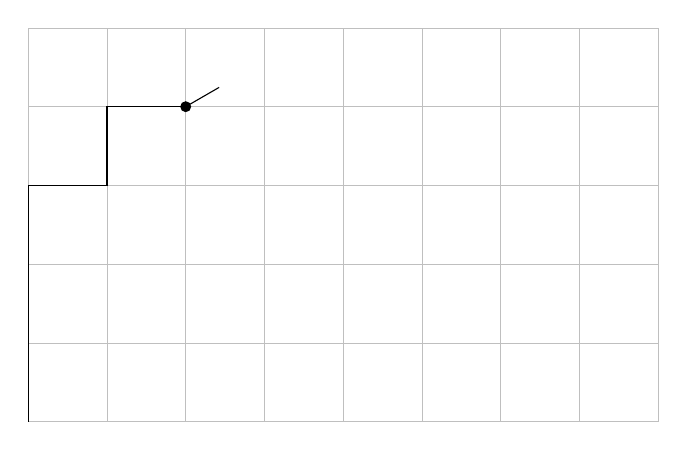
\begin{tikzpicture}[dot/.style={circle,inner sep=1.4pt,fill}]
\draw[very thin, gray!50, step=1 cm](0,0) grid (8,5);
\draw (0,0) -- (0,3) -- (1,3) -- (1,4) --(2,4);
\node [dot] at (2,4) {};
\draw (2,4) -- +(30:0.49);
\end{tikzpicture}
\end{alignedat}
\end{equation}
\quad
\vspace*{-5mm}

%----------------------------------------

\subsection*{Answer}
$p \wedge (q \vee r) = l$. We can write $p \wedge (q \vee r)$ Since this is equilvalent to $l$ (the lamp is on), the current is flowing in the circuit. The circuit represents $p \wedge (q \vee r)$

%%%%%%%%%%%%%%%%%%%%%%%%%%%%%%%%%%%%%%%%%%%%%%%%%%%%%%%%%%%%%%%%


\end{fleqn}
\end{document} 